\subsection{Controleur} %
Le controller est la pour assurer que seul les voitures d'un certains type passe à la fois. Parmis ces voitures il doit limiter le nombre de voiture consécutivfes qui passent pour laisser aux voiture de l'autre type l'occasion de paser.


\subsubsection{Vérification du type de voitures}
Pour ne laisser qu'un seul de type de voiture passer nous avons définis une classe \texttt{Type} qui varie dans l'enssemble: \texttt{[a, b]}. le modèl contient une place \texttt{LastType} qui contient initialment le jeton \texttt{Type.a}.

Comme cité précédement la voiture est en fait un type composé. Ce type est composé d'un numéro de voiture et d'un type de voiture. Pour qu'une voiture puisse avancer, elle doit tirer ce jeton, et ce dernier doit être égale au type de la voiture.

\subsubsection{Vérification capacité du pont}
Le pont ne peut accepter que \texttt{Nalt} voitures à la fois. Pour modéliser cette contrainte nous avons utilisé une classe de type \texttt{Compteur} avec la plage de valeurs suivante: [0;Nalt]. Dans nos exemples nous utilisons \texttt{Nalt = 2}.\\


Nous avons une place \texttt{Position} qui est initialisé avec le jeton \texttt{Counter.0} et qui produit le jeton qu'elle contient, puis récupére le jeton + 1. ainsi la guarde ne laisse passer une voiture que si la place \texttt{Position} ne dépasse  pas une valeur maximum.\\

Voici le modèle du controleur Figure:\ref{fig:ctrl}:\\
Le coeur du controlleur est représenté en rouge.

La transition Dem (de couleur bleu sur la gauche) recoit le jeton de la voiture, si ce jeton satisfait la garde, alors la voiture peut aller sur le pont.

La transition \texttt{leaveLAst} est lié au Pont et au Controleur car elle permet à la dernière voiture de quitter le Pont mais c'est elle qui permet aussi le changement de sens du pont. Cette transition ( \texttt{leaveLast} ) change la place \texttt{LastType} avec l'autre type, remet à zéro le compteur en entré et en sortie du Pont.

\subsubsection{Timeout}
Le timeout est géré par le \texttt{Controlleur}. Nous avons choisi de le représenter sous la forme d'une transition.

Cette transition, pour être tirée doit prendre le jeton de la place \texttt{LastType}, \texttt{Position}, \texttt{Orderer}. en prenant ces jetons, elle renvoie dans chaqcune des place, un compteur = 0 pour les 2 compteurs, et le type suivant pour la palce \texttt{LastType}. Ainsi les voitures venant dans l'autre sens (Aka: l'autre type de voiture) peuvent passer.

Pour assurer la propriété \texttt{P1} cette transition de \texttt{timeout} ne peux être tiré que s'il y a autant de voiture qui sont entrées que de voitures qui sont sorties. ainsi si la transition est tiré c'est qu'il n'y a plus de voitures sur le Pont.

\begin{figure}[ht]
    \centering
    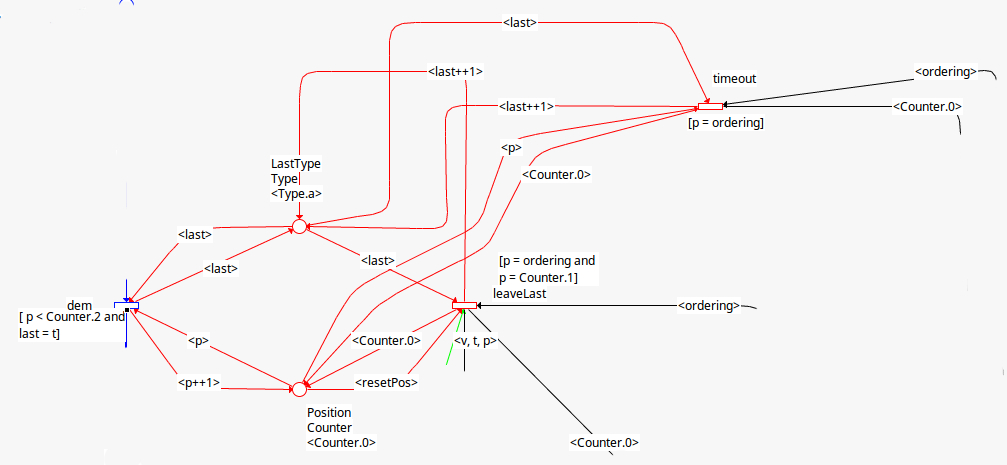
\includegraphics[scale=0.5]{figures/ctrl.jpeg}
    \label{fig:ctrl}
\end{figure}

\newpage

\subsection{Modèle complet} %
Après assemblage des différent composant, on arrive donc au modèle complet suivant Figure \ref{fig:model}:\\

Il pemet donc \texttt{Nalt} voitures de passer de la place \texttt{Start} à la place \texttt{Bridge} en tirant la transition \texttt{dem}. Une fois sur le pont toutes les voitures sauf la dernière vont dans la place \texttt{Outsite} en tirant la tansition \texttt{leave}. La dernière voiture à être entrée sur le pont va aussi dans la place \texttt{Outside} mais cette fois ci en tirant la tansition \texttt{leaveLast}, cette dernière va remettre à zéro les compteurs et laisser les voitures de l'autre type passer.\\

Si par hasard on a: \texttt{Nalt} > nbVoitures, alors même si toutes les voiture d'un type passent, les voitures de l'autre type vont attendre que d'autres voiture arrivent. Du coup c'est à ce moment que le timeout peut ce déclencher (si autant de voitures sont entrée que sorties) et du coup laisser la possibilité au voiture de l'aute type de passer.

\begin{figure}[ht]
    \centering
    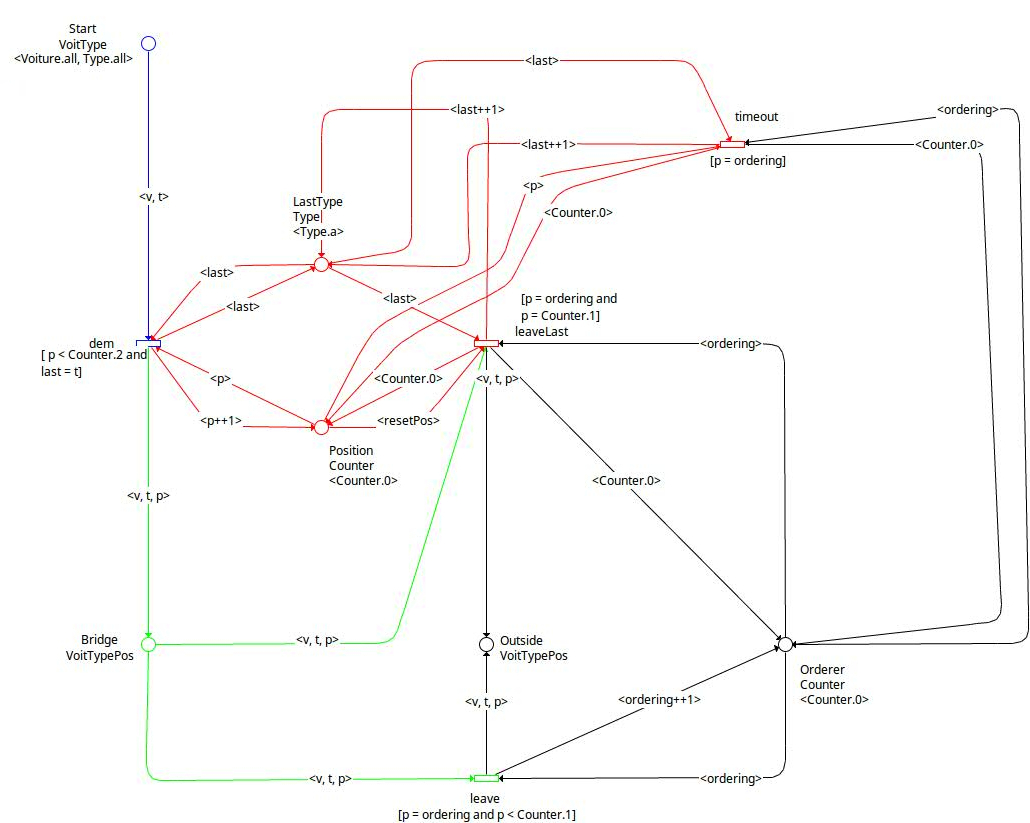
\includegraphics[scale=0.4]{figures/full-model.jpeg}
    \label{fig:model}
\end{figure}

\begin{figure}[ht]
  \centering
  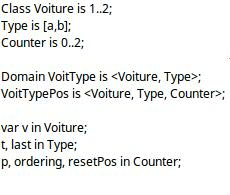
\includegraphics[scale=0.4]{figures/full-model-def.jpeg}
\end{figure}
